% Chapter 2

\chapter{Background} % Main chapter title

\label{Chapter2} % For referencing the chapter elsewhere, use \ref{Chapter2} 


%----------------------------------------------------------------------------------------

\section{Reinforcement Learning}
\label{RL}

\subsection{Markov Decision Processes}
\label{MDP}
Environments in traditional reinforcement learning application are usually modelled as Markov Decision Processes or MDPs.

These can be formulated as systems with the following components:
\begin{itemize}
	\item Finite set of states $S=\{s_0,\ldots,s_n\}$ and actions $A=\{a_0,\ldots,a_m\}$.
	\item A distribution of probabilities $P_a(s,s')$ for transitions from state $s$ to $s'$ for each possible action $a$.
	\item A reward function $R:S\mapsto\mathbb{R}$ for being at a particular state.
	\item The goal in reinforcement learning is to maximise the final reward that an agent achieves in the environment.
\end{itemize}

As the name suggests, MDPs obey the \textit{Markov property}, whereby the probability of the system being in a certain future state exclusively depends upon the present state, and not upon an arbitrarily-long sequence of past states.

In figure~\ref{fig:MDP} we show a sample schematic of a Markov Decision Process, and how states, actions, and rewards could be connected between each other.

\begin{figure}
\centering
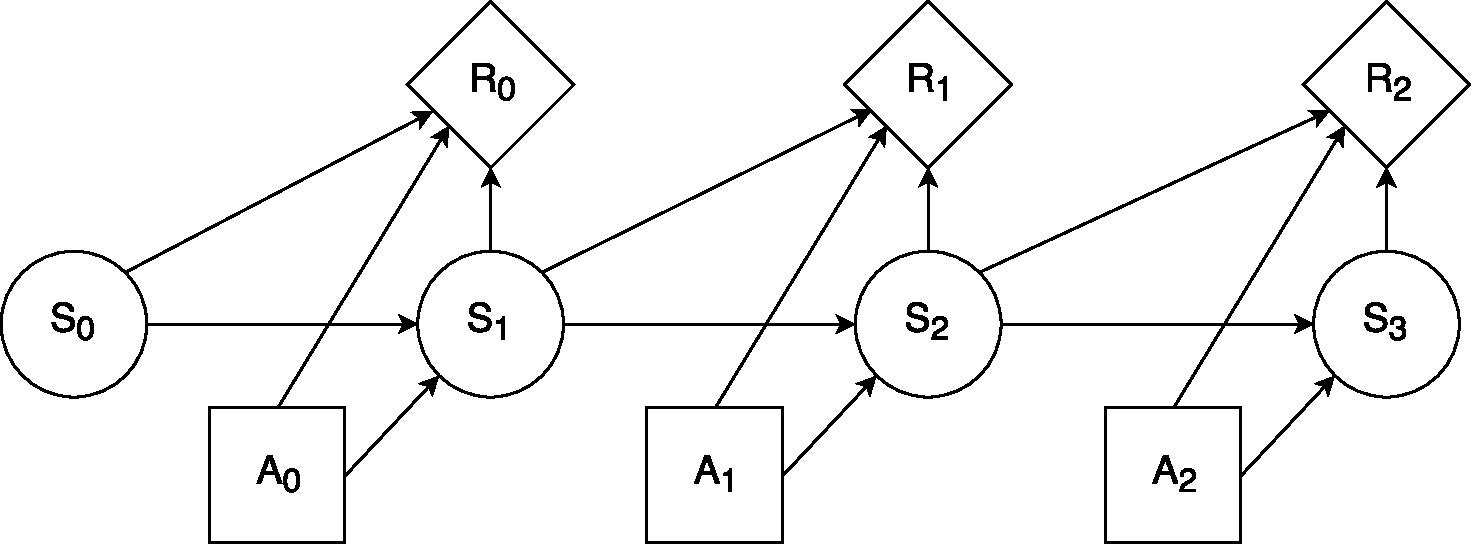
\includegraphics[width=10cm]{Figures/MDP}
\caption{Sample schematic of an MDP.}
\label{fig:MDP}
\end{figure}


\subsection{Q-learning}
\label{qlearning}
Now that we contextualised reinforcement learning environments as Markov Decision Processes, we can introduce the final objective of reinforcement learning tasks: finding a function $\Pi:S\mapsto A$ called \textbf{policy}, that maps the appropriate action $a\in A$ given the current state $s\in S$, as to maximise our agent's final reward.

In particular, we will now present Q-learning \parencite{watkins1992q}.

Q-learning lets us learn the \emph{quality}, or expected utility, of each state-action combination. That is, for each state, we estimate all the expected rewards we obtain by taking each possible action at that particular state. This is represented as a state action table. We can use a Q-table to define a policy by always picking the action with the highest expected return.

More formally, we estimate a function $Q: S \times A \to \mathbb{R}$. We can model $Q$ as a mapping table (initialised with some uniform values), whose value we update at each time step of our simulations.

Here's how we update our Q-table at each time step $t$:
\begin{equation} \label{eq:QlearningUpdate}
  Q(s_{t},a_{t}) = \underbrace{Q(s_t,a_t)}_{\rm old~value} +
  \underbrace{\alpha}_{\rm learning~rate} \times \left[
    \overbrace{\underbrace{r_{t+1}}_{\rm reward} + \underbrace{\gamma}_{\rm
        discount~factor} \underbrace{\max_{a}Q(s_{t+1}, a)}_{\rm
        estimate~of~optimal~future~value}}^{\rm learned~value} -
    \underbrace{Q(s_t,a_t)}_{\rm old~value} \right]
\end{equation}

where:
\begin{itemize}
	\item $\alpha\in[0,1]$ is the \emph{learning rate}, a coefficient that regulates how much the newly learned values will contribute in the update
	\item $\gamma\in[0,1]$ is the \emph{discount factor}, a coefficient that controls the weight of future rewards. Values closer to 0 will make our agent "short-sighted", considering only the immediate rewards.
\end{itemize}

What is our optimal policy when we do Q-learning then? After training, it is simply that function $\pi: S \to A$ that, for each state, returns the action with maximum expected utility in our Q-table.

Algorithm~\ref{alg:Qlearning} reports the pseudocode for Q-learning.

\begin{algorithm}
\caption{Q-learning}
\label{alg:Qlearning}
\begin{algorithmic}[1]
\Require $n$, number of episodes to run Q-learning
\Require $\epsilon$, probability to take random action, rather than follow policy
\Procedure{Q-Learning} {}
\\Initialize $Q(s,a)$ arbitrarily
\For{each episode}
\\ \qquad Initialize $s$
\For{each step of episode}
\\ \qquad \qquad Choose $a_t$ from $s_t$ using policy derived from $Q$ with $\epsilon$-Greedy
\\ \qquad \qquad Take action $a_t$, observe $u$ and $s_{t+1}$
\\ \qquad \qquad Update Q-table using equation~\ref{eq:QlearningUpdate}
\EndFor
\EndFor
\EndProcedure
\end{algorithmic}
\end{algorithm}

From this procedure we need to highlight two important concepts.

The first one is the concept of episode, which is defined as a sequence of actions in which an agent (the algorithm) interacts with its environment until it reaches a certain terminal. In Q-learning we need to specify a certain number of episodes that we will run the algorithm for. The more episodes we choose, that more optimal the policy is likely to be, since the has more interactions with its environment.

The second concept is that of $\epsilon$-greedy, which we introduce in the next subsection on the tradeoff in Reinforcement Learning between exploration and exploitation.

\subsection{Exploration/Exploitation tradeoff}
An important theme in reinforcement learning, and that we also focus our attention on in our project is the idea of the tradeoff between Exploration and Exploitation.

In reinforcement learning, and generally in decision making, we have a fundamental choice: \textit{exploitation}, whereby you make the best decision given current information, or \textit{exploration}, where we prefer gather more information.

The reason why this is a trade-off is because the best long-term strategy may involve short-term sacrifices, so we wish to gather enough information to make the best overall decisions.

For example, consider the case where we need to choose a restaurant for dinner. We can either go to our favourite restaurant (exploitation), or we could choose to try a new restaurant (exploration) with the hope that it is eventually better than our favourite, but also risking that it is worse.

In reinforcement learning this usually can be represented as an $\epsilon$-greedy approach. In this approach, we choose to either \textit{exploit} our current knowledge and choose the action $a_t^*$ that we think is optimal given what we currently know, or we choose to \textit{explore} by taking a random action.

\[
a_t =
\left\{
	\begin{array}{ll}
		a_t^*   & \mbox{with probability 1-$\epsilon$}\\
		\text{random action} & \mbox{with probability $\epsilon$}
	\end{array}
\right.
\]

It is critical to account for this tradeoff when developing algorithms in reinforcement learning, and we will show how we can still keep allow for both exploration and exploitation with the techniques that we develop.

\subsection{Deep Reinforcement Learning}
\subsubsection{DQN}
% Add DQN
%\subsection{Problems with reinforcement learning techniques}
%\subsection{Actor critic}

%----------------------------------------------------------------------------------------

\section{Generative Adversarial Networks}
\label{sec:gan}
Generative Adversarial Networks, or GANs, are a deep neural network architecture composed of two neural networks, set against each other (thus "adversarial").

GANs were introduced in a paper by \cite{goodfellow2014generative}. Yann LeCun, Facebook's AI Research director referred GANs as being "the most interesting idea in the last 10 years in ML".

What have made GANs particularly successful in past work is their ability to model any distribution of data, and provide, after training, both a generative model and a discriminative model based on the initial distribution of the data. Let us define what we mean by these terms.

A \textit{generative} model is one that is able to produce new data points that fit the distribution of the training data. For example, a Gaussian Mixture Model is a model that, after training, could generate new data based on the original distribution. More formally, training a generative model can be seen as maximum likelihood estimation problem:

\[\mathscr{L} = \prod_{i=1}^{m} p_{model}(x_i;\theta)\]

More specifically, we want to maximise the likelihood that a sample $x$ that the generative model produces belongs to the distribution of our initial data.

A \textit{discriminative} model is one that can discern (or "discriminate") the difference between two (or more) classes/labels. For example, we could train a Convolutional Neural Network that is able to tell us whether an input image is a face (1) or not (0).

Depending on the task at hand, we may be more interested in the generative model (for example in the case of image synthesis), or in the discriminative model, or in both.

Next, we will look at the typical architecture of Generative Adversarial Networks.

\subsection{Architecture of GANs}
Since GANs were introduced in 2014, many variants of GANs spawned from the research community. Here we will focus on the architecture of the original, vanilla GAN.

All variations of GANs will nevertheless contain two main components, which are both modelled as neural networks. These two models are trained simultaneously. One is the \emph{generator} model, that takes an input \emph{z} and produces a sample \emph{x} from an implicit probability distribution. The other is the \emph{discriminator}, a classifier that, given a sample, tries to identify it as originating from the generator model or from the original distribution.

An intuition to this set up is the following: the generator \code{G} can be imagined as a counterfeiter trying to produce fake banknotes or paper money; the discriminator \code{D} is the police, trying to distinguish real banknotes from the fake ones generated by the counterfeiter. As the counterfeiter becomes better and better at producing banknotes, the police will also try to improve its counterfeiting techniques.

More formally, \code{G} is a differentiable function whose parameters are trained to minimise correct assignments of \code{D}. \code{D} is also a differentiable function, which has been trained to maximise correct labels to the real and the fake samples.

In figure~\ref{fig:VanillaGAN} summarises this whole procedure by showing the architecture of GANs.

At each iteration, the mini-batch inputs to the discriminator \code{D} are taken from both the real data sampled from the training data, and the samples generated by the generator, whose inputs is random latent variable $z$. Given \code{D}'s prediction, we then apply a gradient-based optimisation method to update both \code{D}'s and \code{G}'s parameter.

To do so, we follow the loss function that defined based on the goals of each network. This cost function implicitly models a zero-sum game, which in game theory are guaranteed to achieve an equilibrium, by the minimax theorem \citep{du2013minimax}.

The cost function for the whole system would look like the following minimax game:
\[\min_{G} \max_{D} V(G, D) = \mathbb{E}_{x\sim p_{data}(x)}[log D(x)] + \mathbb{E}_{z \sim p_{g}(z)}[log(1-D(G(z)))] \]

\begin{figure}
\centering
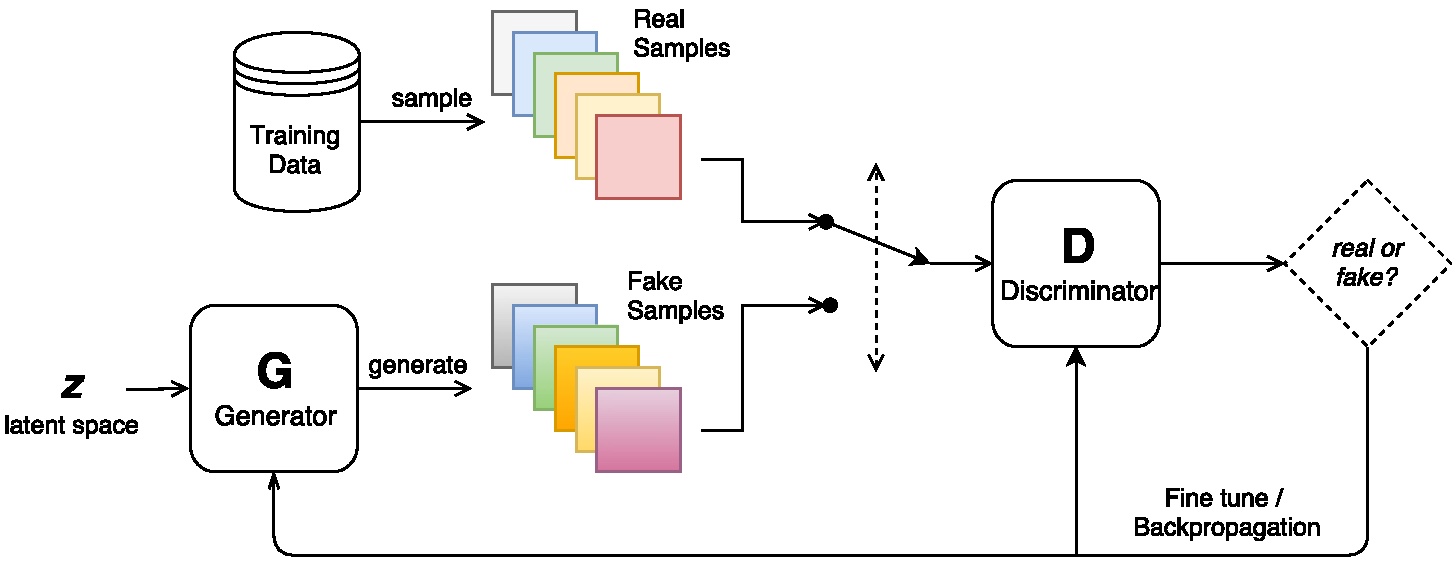
\includegraphics[width=15cm]{Figures/VanillaGAN}
\caption{Architecture of a Generative Adversarial Network}
\label{fig:VanillaGAN}
\end{figure}

\subsection{Successes}
\label{successes}
\subsubsection{DCGAN}
% TODO: DCGAN

%\subsection{Conditional GANs}

%----------------------------------------------------------------------------------------

\section{Related work}
\subsection{Reinforcement learning with unsupervised auxiliary tasks}
There have few successes in transferring deep reinforcement learning across domains. Mostly notably, \cite{jaderberg2016reinforcement} introduced a technique to identify in an unsupervised way, multiple pseudo-reward functions based on all training signals that the agent collected as observations. While doing deep reinforcement learning, therefore, \citeauthor{jaderberg2016reinforcement} would not only try to directly maximise the agent's cumulative reward, but also all the identified extrinsic rewards. 

There is a potential to re-use these identified extrinsic rewards in other domains, but this is an indirect way to tackle the problem of transferring behaviour. 

In this work, they would first identify what auxiliary rewards the observations can give, to then reuse them on different task. Also, we have little to no control to guide the unsupervised exploration of auxiliary rewards functions towards a related task that we have the power to define.

In fairness, \citeauthor{jaderberg2016reinforcement} introduced auxiliary rewards as a way to speed up reinforcement learning on a single task, rather than aiming to transfer these to related tasks.

In our work we do not indirectly try to capture pseudo-rewards given a task, but we try to capture transferrable knowledge directly from the training policies.


\subsection{Generative Adversarial Imitation Learning}

An analogous way to do transfer learning in the context of reinforcement learning imitation learning, an important subfield of research in the reinforcement learning community. Imitation learning, as the name suggests, mostly deals with training agents that imitate an expert behaviour. 

It does so by taking signals coming in from experts, usually encoded human behaviour. Having such signals can significantly decrease training time, as well as provide new insight onto different optimal behaviour that could achieve better rewards. Most notably, researchers at OpenAI used signals from professional Go players to build imitation learning techniques \citep{silver2016mastering}. This was only used as a priming step to learning the game of Go, and was used in combination with Deep Q-networks.

Generally, the imitating agent is trained on the same environment as the expert agent. Thus, imitation learning, while still being a form of knowledge transfer, only relates to techniques that do not cross task domains.

Despite this crucial difference with what the goal of our project, a particular technique that has been recently introduced for imitation learning is still very much related to some of the components of our pipeline.

Generative Adversarial Imitation Learning \citep{ho2016generative} or GAIL bases much of its architecture on GANs.

\citeauthor{ho2016generative} from OpenAI introduced it as a better-performing alternative to imitation learning techniques. In particular, they motivated their work on the computational cost of a typical approach to imitation learning, which does not directly train a policy that is imitating an expert.
In fact, one way to do imitation learning was to use inverse reinforcement learning on the expert policy to obtain its reward function. Based on this reward function, reinforcement learning techniques could be used to train imitating agent. Given this pipeline, we can notice that it is an indirect way of conducting imitation learning, which is prone to produce a model that does not accurately represent the distribution of trajectories of the agent.

With GAIL there is no need to extract a reward function, but they let the Generative Adversarial Network capture the distribution of observations and action pairs. After training the GAN, the Generator will have been trained to produce appropriate actions, given observations. The real data that the GAN is trained with are trajectories coming in from the expert policy. Algorithm~\ref{alg:gail} also shows a simplified algorithm for GAIL.

In figure~\ref{fig:GAIL-GAN} we present a schematic of each component involved in training a Generative Adversarial Network for Imitation Learning. We notice right away that the GAIL architecture closely resembles the Vanilla GAN, as we showed in figure~\ref{fig:VanillaGAN}. After training, the Generator will represent the imitating policy, which will hopefully perform as well as the expert policy. Again, there is no need to extract a reward function in this whole pipeline.

In this work, \citeauthor{ho2016generative} have shown groundbreaking results in imitation learning using GANs, as they achieved much better performances with traditional imitation learning techniques like Behavioural Cloning or Dataset Aggregation.

In our work, we aim to achieve as great results in transferring knowledge across domains.

\begin{algorithm}[tb]
    \caption{Generative adversarial imitation learning}
    \label{alg:gail}
    \begin{algorithmic}[1]
       \State {\bfseries Input:} Expert trajectories $\tau_E \sim \pi_E$, initial policy and discriminator parameters $\theta_0, w_0$
       \For{$i = 0, 1, 2, \dotsc$}
           \State Sample trajectories $\tau_i \sim \pi_{\theta_i}$
           \State Update the discriminator parameters from $w_i$ to $w_{i+1}$ with the gradient
           \State Take a policy step from $\theta_i$ to $\theta_{i+1}$, using the TRPO/PPO rule.
        \EndFor
    \end{algorithmic}
\end{algorithm}

\begin{figure*}
\centering
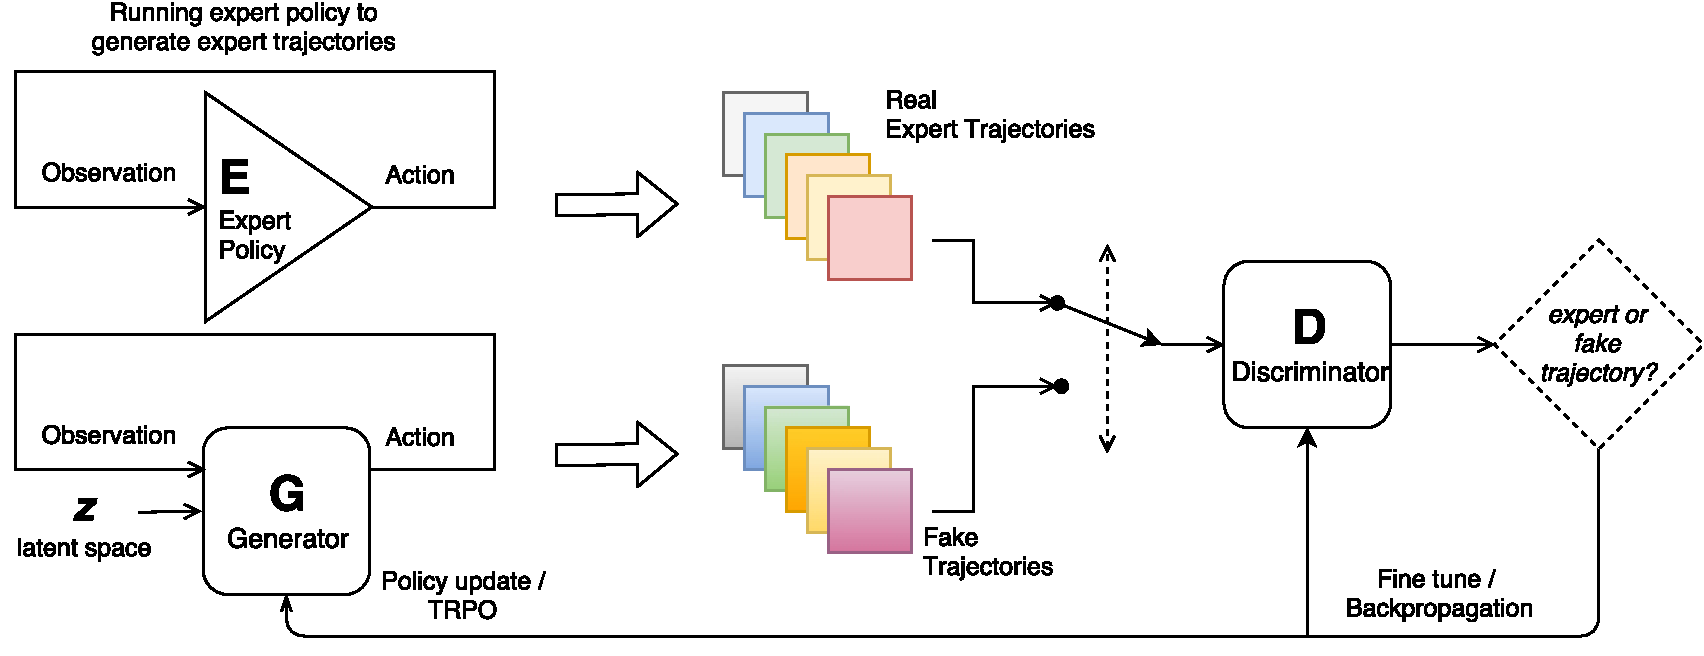
\includegraphics[width=15cm]{Figures/GAIL-GAN}
\caption{Generative Adversarial Imitation Learning (GAIL) architecture}
\label{fig:GAIL-GAN}
\end{figure*}%----------------------------------------------------------------------------------------